On considère le cube $ABCDEFGH$ donné ci-dessous.

\begin{center}
	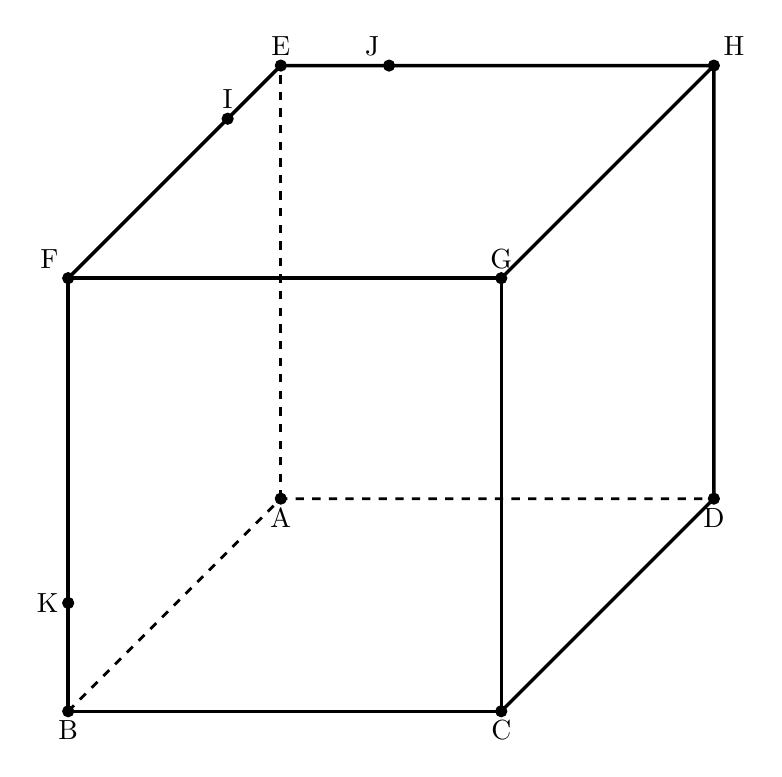
\begin{tikzpicture}[line join=bevel]
		\draw[line width=1.25pt] (0.5,0.5)rectangle (6,6) ; %BCGF
		\draw[line width=1.25pt] (6,0.5)--(8.7,3.2)--(8.7,8.7)--(6,6) ;%CDHG
		\draw[line width=1.25pt] (8.7,8.7)--(3.2,8.7)--(0.5,6) ;%HEF
		\draw[line width=1pt,dashed] (0.5,0.5)--(3.2,3.2)--(8.7,3.2) ;%BAD
		\draw[line width=1pt,dashed] (3.2,3.2)--(3.2,8.7) ;%AE
		\foreach \Coord/\Sommet/\Pos in {(3.2,3.2)/A/below,(0.5,0.5)/B/below,(6,0.5)/C/below,(8.7,3.2)/D/below,(3.2,8.7)/E/above,(0.5,6)/F/above left,(6,6)/G/above,(8.7,8.7)/H/above right,(2.525,8.025)/I/above,(4.575,8.7)/J/above left,(0.5,1.875)/K/left}
		\filldraw \Coord circle[radius=2pt] node[\Pos] {\Sommet} ;
	\end{tikzpicture}
\end{center}

On donne trois points $I$, $J$ et $K$ vérifiant : \[\vect{\text{RI}} = \dfrac{1}{4} \vect{\text{EH}},\qquad   \vect{\text{EJ}} = \dfrac{1}{4}  \vect{\text{EF}}, \qquad  \vect{\text{BK}} = \dfrac{1}{4}  \vect{\text{BF}}.\]
%
Les points $I$, $J$ et $K$ sont représentés sur la figure donnée en annexe, à compléter et à rendre avec la copie.

On se place dans le repère orthonormé $\left(\text{A};\vect{\text{AB}},\vect{\text{AD}},\vect{\text{AE}}\right)$.

\begin{enumerate}
	\item Donner sans justification les coordonnées des points $I$, $J$ et $K$.
	\item Démontrer que le vecteur $\vect{\text{AG}}$ est normal au plan $(IJK)$.
	\item Montrer qu'une équation cartésienne du plan $(IJK)$ est $4x + 4y + 4z - 5 = 0$.
	\item Déterminer une représentation paramétrique de la droite $(BC)$.
	\item En déduire les coordonnées du point $L$, point d'intersection de la droite $(BC)$ avec le plan $(IJK)$.
	\item Sur la figure en annexe, placer le point $L$ et construire l'intersection du plan $(IJK)$ avec la face $(BCGF)$.
	\item Soit M$\left(\frac{1}{4};1;0\right)$. Montrer que les points $I$, $J$, $L$ et $M$ sont coplanaires.
\end{enumerate}

